\documentclass[11pt]{article}
\usepackage[margin=1in]{geometry}
\usepackage{amsmath,amssymb,booktabs,array,graphicx,float}
\usepackage[hidelinks]{hyperref}
\usepackage{caption}
\captionsetup{font=small,labelfont=bf}
\graphicspath{{./}}
\setlength{\parindent}{0pt}
\setlength{\parskip}{6pt}

\title{\vspace{-2em}Tripartite Space Cybersecurity Resilience Model:\\
Computed Results, Figures, and Tables}
\author{Abebe Diro \and Angela An \and Abera Tullu}
\date{Generated from live model output}

\begin{document}
\maketitle

\noindent All values below are live output from the reference
implementation (calibrated parameter set; finite-adversary cap active;
$n=63$ disclosed incident corpus; 10-fold cross-validation with seed 42).
Figures are vector PDFs produced by the analysis pipeline. Tables are
emitted by \texttt{make\_tables.py} and reproduce the paper's Table~V--VII
family with recomputed numbers.

\section{Result Tables}
% ===== Table: Baseline Resilience Trajectory (live model output) =====
\begin{table}[H]
\centering
\caption{Baseline Resilience Trajectory (Model-Conditional)}
\label{tab:baseline_live}
\scriptsize
\renewcommand{\arraystretch}{1.15}
\begin{tabular}{ccccc}
\toprule
\textbf{Year} & \textbf{$R_{sys}$} & \textbf{$R_{eff}$} & \textbf{Threat} & \textbf{Erosion} \\
\midrule
0 & 0.283 & 0.283 & 0.100 & 0.0\% \\
3 & 0.635 & 0.599 & 0.248 & 5.8\% \\
5 & 0.726 & 0.658 & 0.343 & 9.5\% \\
8 & 0.810 & 0.699 & 0.451 & 13.7\% \\
10 & 0.864 & 0.728 & 0.503 & 15.7\% \\
15 & 0.917 & 0.746 & 0.580 & 18.6\% \\
20 & 0.928 & 0.744 & 0.609 & 19.8\% \\
\bottomrule
\end{tabular}
\end{table}

% ===== Table: Comparative Performance on disclosed corpus (live) =====
\begin{table}[H]
\centering
\caption{Comparative Performance Against Baseline Models (10-fold CV, disclosed $n=63$)}
\label{tab:validation_live}
\scriptsize
\renewcommand{\arraystretch}{1.15}
\begin{tabular}{lccc}
\toprule
\textbf{Model} & \textbf{RMSE} & \textbf{$r$} & \textbf{MAPE} \\
\midrule
Naive mean & 0.180 & -0.44 & 34.2\% \\
Static risk (FAIR) & 0.373 & 0.86 & 64.9\% \\
Resilience triangle & 0.142 & 0.99 & 24.6\% \\
Linear additive & 0.076 & 0.90 & 12.3\% \\
Independent dimensions & 0.101 & 0.82 & 11.9\% \\
\textbf{Proposed (full)} & \textbf{0.064} & \textbf{0.93} & \textbf{10.0\%} \\
\bottomrule
\end{tabular}
\end{table}

% ===== Table: Strategy performance (live) =====
\begin{table}[H]
\centering
\caption{Strategy Performance at Year 10 (Model-Conditional)}
\label{tab:strategy_live}
\scriptsize
\renewcommand{\arraystretch}{1.15}
\begin{tabular}{lccc}
\toprule
\textbf{Strategy} & \textbf{$R_{sys}$ (yr10)} & \textbf{$R_{eff}$ (yr10)} & \textbf{$\Delta$ vs base} \\
\midrule
Baseline & 0.864 & 0.728 & -- \\
Preparedness & 0.877 & 0.739 & +1.4\% \\
Resistance & 0.828 & 0.701 & -3.7\% \\
Restoration & 0.874 & 0.736 & +1.0\% \\
Adaptation & 0.867 & 0.731 & +0.4\% \\
Supply Chain & 0.874 & 0.736 & +1.0\% \\
\textbf{Holistic} & \textbf{0.932} & \textbf{0.777} & \textbf{+6.7\%} \\
\bottomrule
\end{tabular}
\end{table}

% ===== Table: Sobol sensitivity indices (live) =====
\begin{table}[H]
\centering
\caption{Parameter Sensitivity (Sobol Indices, Year 10)}
\label{tab:sobol_live}
\scriptsize
\renewcommand{\arraystretch}{1.15}
\begin{tabular}{clcc}
\toprule
\textbf{\#} & \textbf{Parameter} & \textbf{$S_i$} & \textbf{$S_{Ti}$} \\
\midrule
1 & $gamma\_threat$ & 0.489 & 0.504 \\
2 & $theta$ & 0.269 & 0.272 \\
3 & $k\_restore$ & 0.081 & 0.081 \\
4 & $delta\_threat$ & 0.056 & 0.058 \\
5 & $k\_supply$ & 0.031 & 0.032 \\
6 & $beta$ & 0.024 & 0.023 \\
7 & $phi$ & 0.015 & 0.012 \\
8 & $k\_prep$ & 0.009 & 0.012 \\
\bottomrule
\end{tabular}
\end{table}

% ===== Table: Operational constraint scenarios (live) =====
\begin{table}[H]
\centering
\caption{Operational-Constraint Scenario Effects (C1--C3)}
\label{tab:constraints_live}
\scriptsize
\renewcommand{\arraystretch}{1.15}
\begin{tabular}{llc}
\toprule
\textbf{Constraint} & \textbf{Metric} & \textbf{Value} \\
\midrule
Reference & Holistic advantage (yr10) & 6.7\% \\
C1 budget & Holistic advantage (yr10) & 7.6\% \\
C2 cap (0.85) & Erosion (yr20) & 17.9\% \\
C2 cap (0.85) & Tax mult.\ yr20 (capped) & 1.22$\times$ \\
C2 uncapped & Tax mult.\ yr20 & 1.54$\times$ \\
C3 ($T_{cyc}{=}5$) & Mean resilience gain & +0.3\% \\
C3 ($T_{cyc}{=}5$) & Cumulative cost & +22.0\% \\
\bottomrule
\end{tabular}
\end{table}

% ===== Table: Prior-perturbation robustness (live) =====
\begin{table}[H]
\centering
\caption{Year-10 Policy Conclusions under Adverse Prior Perturbation}
\label{tab:perturbation_live}
\scriptsize
\renewcommand{\arraystretch}{1.15}
\begin{tabular}{lcc}
\toprule
\textbf{Conclusion} & \textbf{Baseline} & \textbf{Adverse Shift} \\
\midrule
Holistic advantage & 6.7\% & 6.7\% \\
Supply-chain leverage $L$ & 1.71 & 1.71 \\
Red Queen erosion & 15.7\% & 18.2\% \\
\bottomrule
\end{tabular}
\end{table}

% ===== Table: Case-study posture indices (live) =====
\begin{table}[H]
\centering
\caption{Retrodictive Case-Study Posture Indices}
\label{tab:cases_live}
\scriptsize
\renewcommand{\arraystretch}{1.15}
\begin{tabular}{lcp{3.4cm}}
\toprule
\textbf{Case} & \textbf{AHP Posture} & \textbf{Observed Outcome} \\
\midrule
Viasat KA-SAT (2022) & 0.272 & Catastrophic; $\approx$45-day physical recovery \\
Starlink (2022) & 0.472 & Localized; days-scale disruption \\
\bottomrule
\end{tabular}
\end{table}

% ===== Table: Calibrated parameter set (Table V) =====
\begin{table}[H]
\centering
\caption{Calibrated Parameter Set with Uncertainty and Identifiability Class}
\label{tab:params_live}
\scriptsize
\renewcommand{\arraystretch}{1.1}
\begin{tabular}{llccl}
\toprule
\textbf{Parameter} & \textbf{Sym.} & \textbf{Value} & \textbf{80\% CI} & \textbf{Class} \\
\midrule
Preparedness decay & $k\_prep$ & 0.05 & [0.035, 0.065] & Practical \\
Resistance decay & $k\_resist$ & 0.07 & [0.049, 0.091] & Practical \\
Restoration decay & $k\_restore$ & 0.12 & [0.084, 0.156] & Structural \\
Adaptation decay & $k\_adapt$ & 0.03 & [0.021, 0.039] & Structural \\
Supply chain decay & $k\_supply$ & 0.11 & [0.077, 0.143] & Practical \\
Latency sensitivity & $alpha$ & 0.85 & [0.6, 1.11] & Practical \\
Inaccessibility & $beta$ & 1.2 & [0.84, 1.56] & Practical \\
Radiation sensitivity & $gamma$ & 0.9 & [0.63, 1.17] & Practical \\
Thermal sensitivity & $gamma\_T$ & 0.15 & [0.1, 0.2] & Weak \\
Superlinear exponent & $mu$ & 0.8 & [0.56, 1.04] & Structural \\
Adversary learning & $theta$ & 0.12 & [0.084, 0.156] & Practical \\
Adversary amplification & $phi$ & 0.25 & [0.17, 0.33] & Structural \\
Threat decay & $delta\_threat$ & 0.08 & [0.056, 0.104] & Structural \\
Max threat impact & $gamma\_threat$ & 0.35 & [0.25, 0.46] & Structural \\
Min threat capability & $S\_threat\_min$ & 0.1 & [0.07, 0.13] & Practical \\
SC risk sensitivity & $eta$ & 0.45 & [0.32, 0.58] & Weak \\
Complexity sensitivity & $nu$ & 0.3 & [0.21, 0.39] & Weak \\
\bottomrule
\end{tabular}
\end{table}


\clearpage
\section{Figures}

\begin{figure}[H]\centering
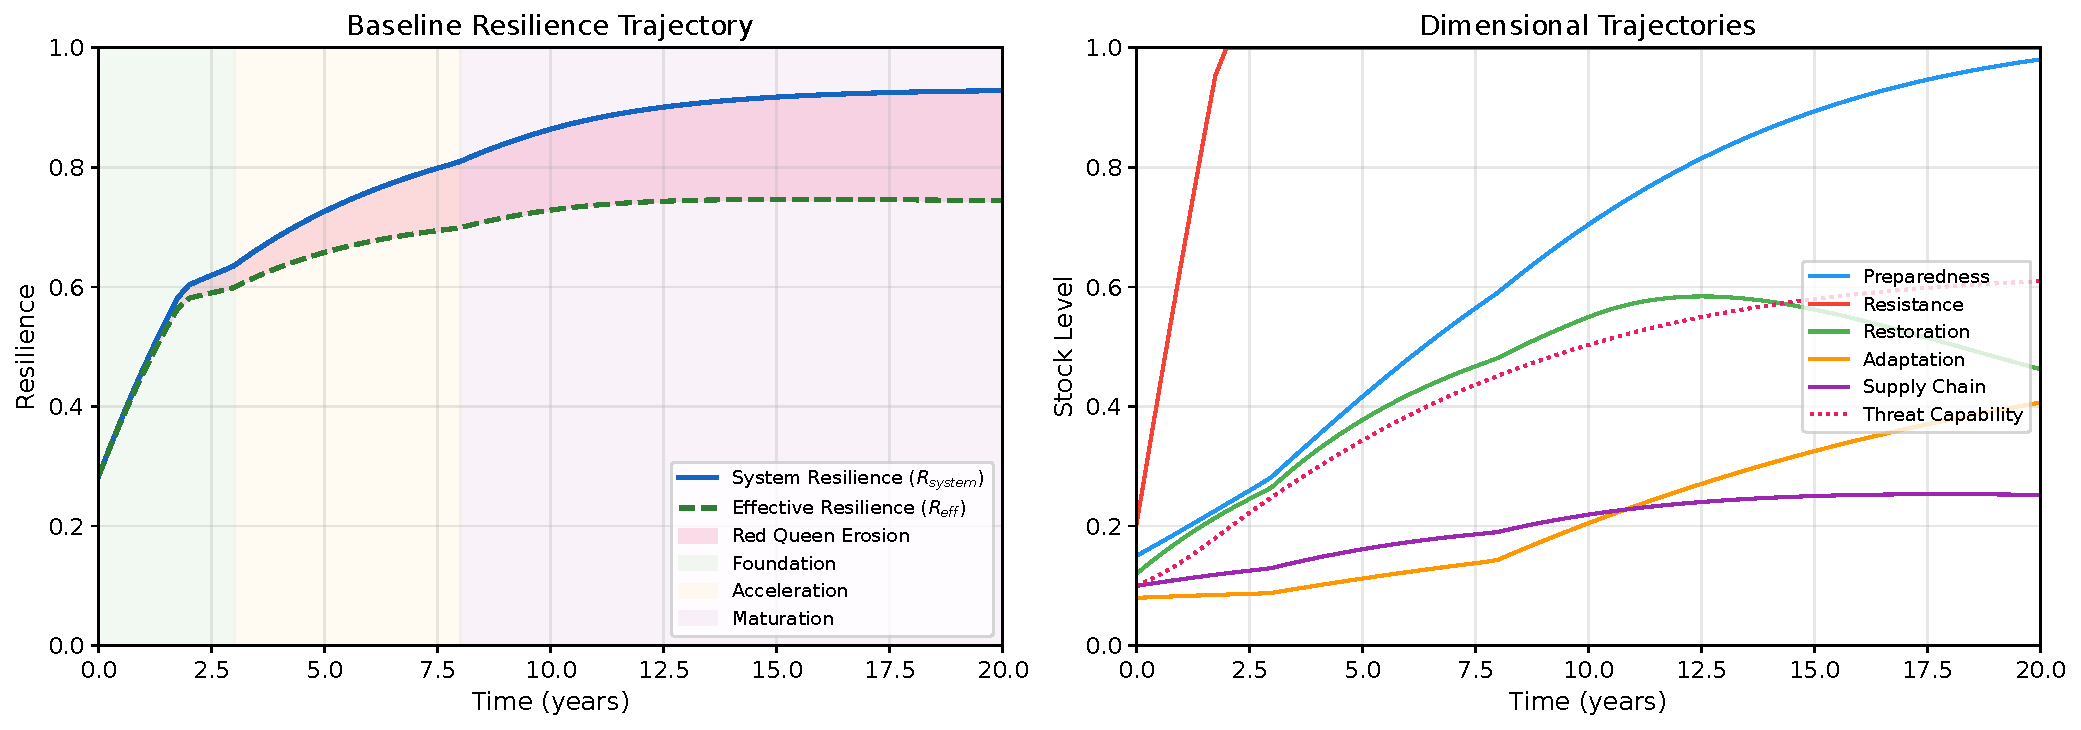
\includegraphics[width=0.82\textwidth]{baseline_trajectory.pdf}
\caption{Baseline resilience trajectory with credible intervals; three
growth phases (foundation, acceleration, maturation) annotated.}
\end{figure}

\begin{figure}[H]\centering
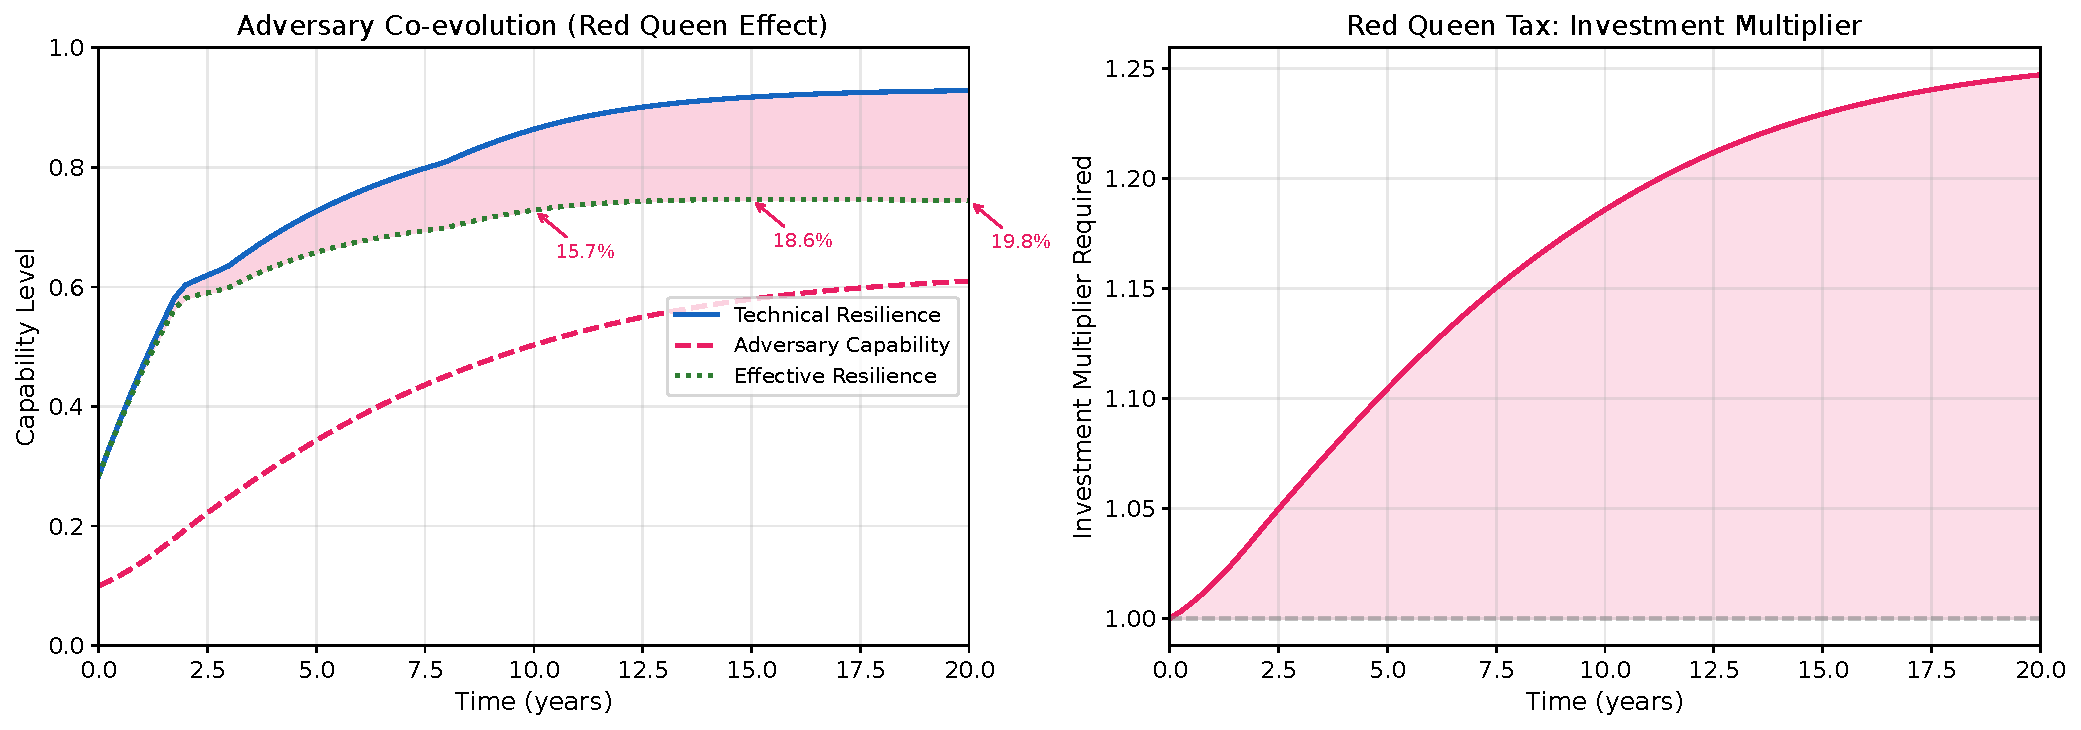
\includegraphics[width=0.82\textwidth]{adversary_dynamics.pdf}
\caption{Technical vs.\ effective resilience under adversary co-evolution;
Red Queen erosion shaded, annotated at years 10 and 20.}
\end{figure}

\begin{figure}[H]\centering
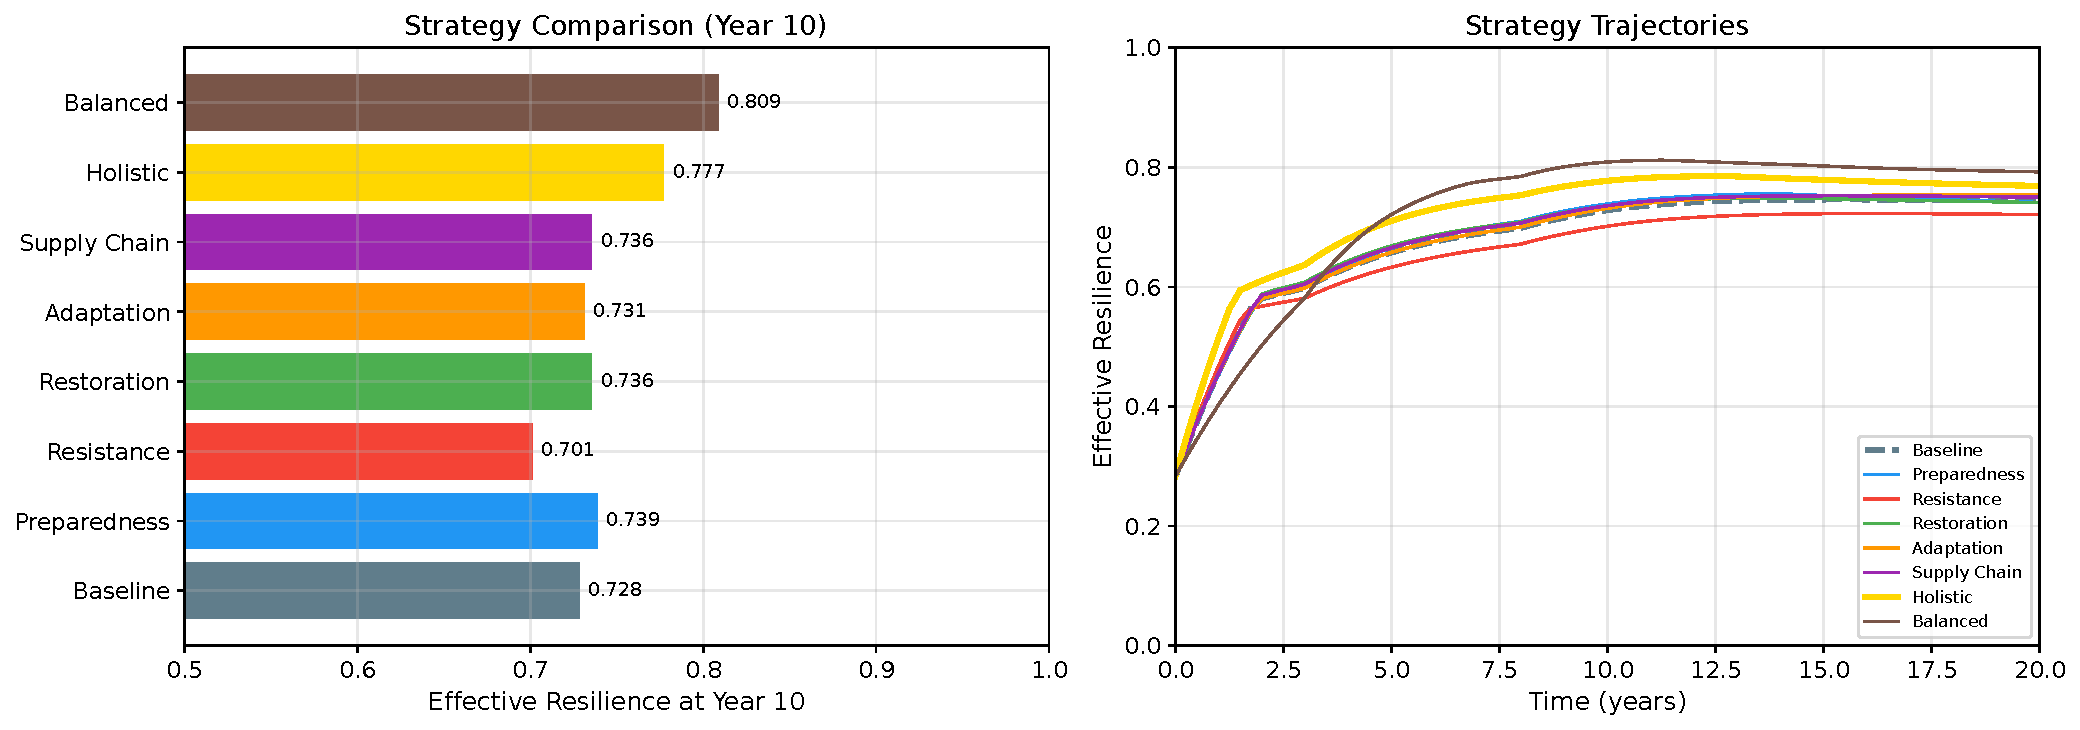
\includegraphics[width=0.82\textwidth]{strategy_comparison.pdf}
\caption{Strategy comparison: holistic vs.\ specialized single-dimension
allocations over the mission lifecycle.}
\end{figure}

\begin{figure}[H]\centering
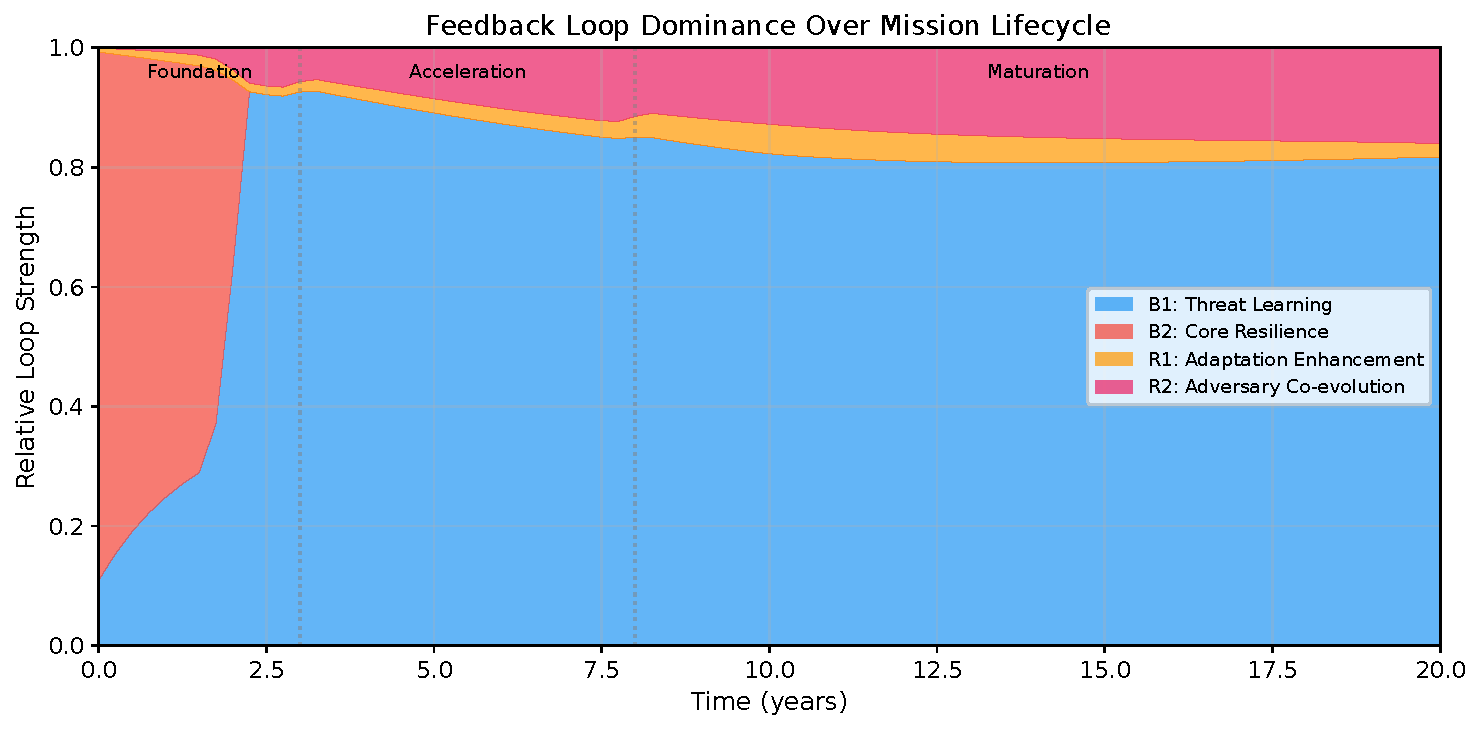
\includegraphics[width=0.82\textwidth]{feedback_loop_dominance.pdf}
\caption{Feedback-loop dominance (B1, B2, R1, R2) over the mission
lifecycle, producing the Red Queen plateau.}
\end{figure}

\clearpage
\begin{figure}[H]\centering
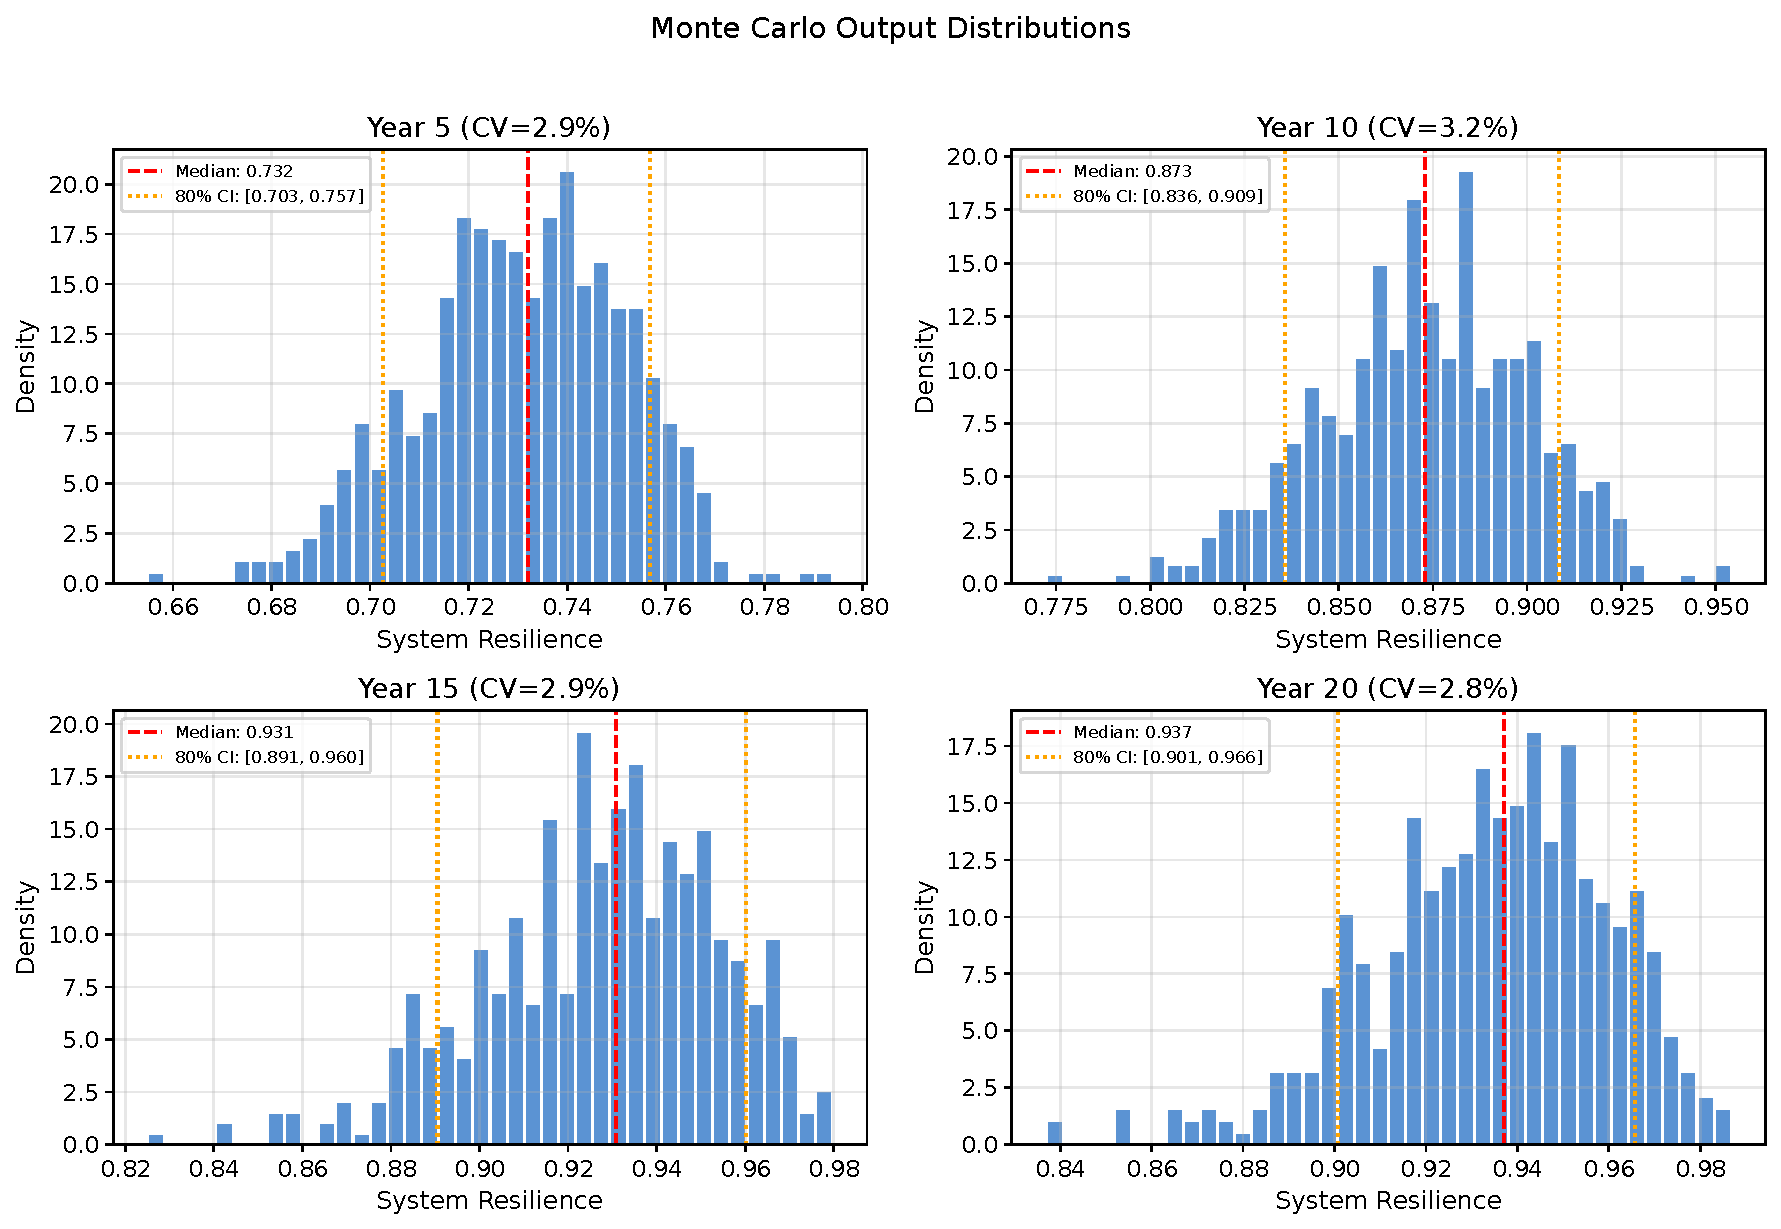
\includegraphics[width=0.82\textwidth]{monte_carlo_distributions.pdf}
\caption{Monte Carlo output distributions for system resilience at years
5, 10, 15, and 20.}
\end{figure}

\begin{figure}[H]\centering
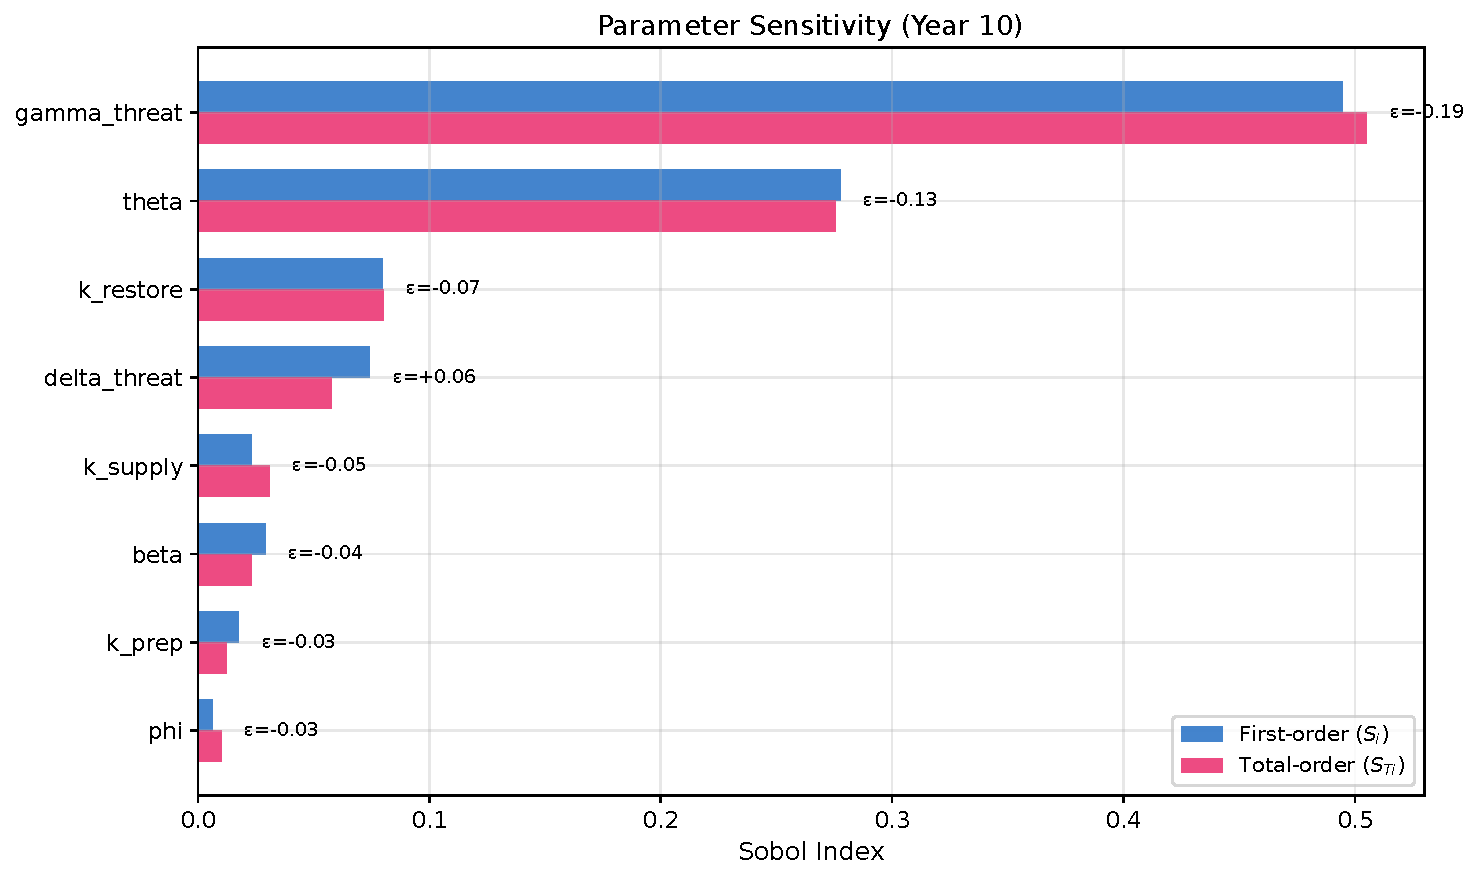
\includegraphics[width=0.82\textwidth]{sensitivity_tornado.pdf}
\caption{Parameter sensitivity: first- and total-order Sobol indices at
year 10.}
\end{figure}

\begin{figure}[H]\centering
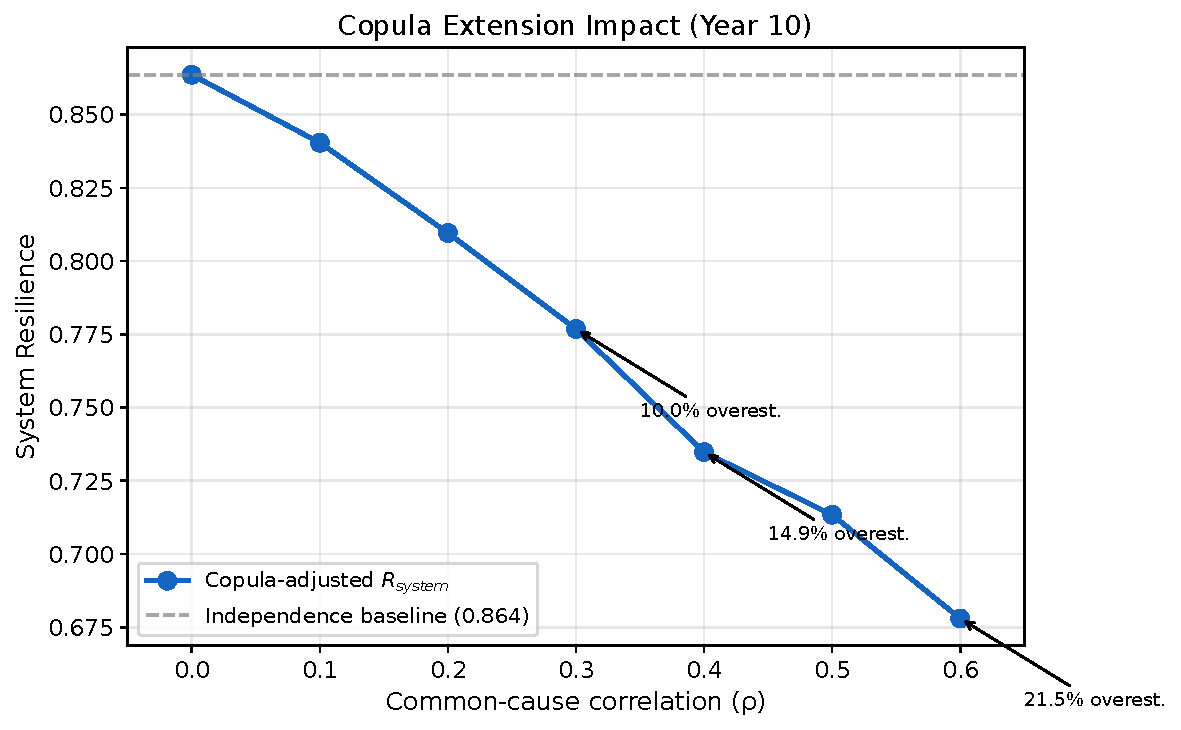
\includegraphics[width=0.82\textwidth]{copula_analysis.pdf}
\caption{Copula-based correlated-failure analysis across
$\rho\in[0,0.6]$.}
\end{figure}

\clearpage
\begin{figure}[H]\centering
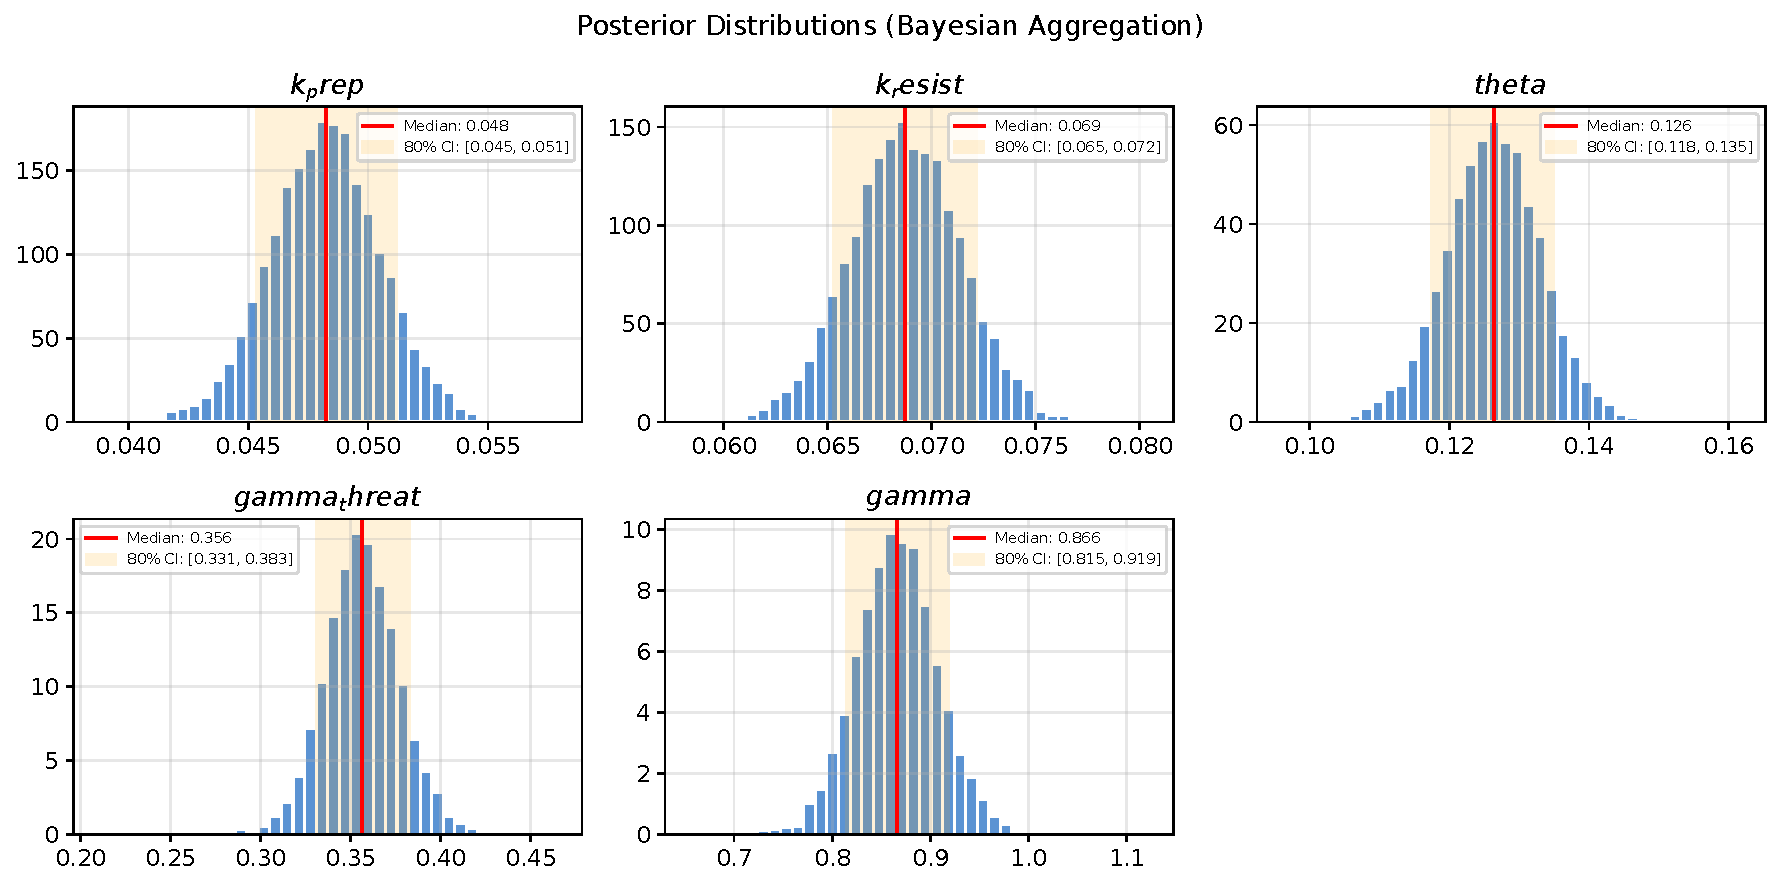
\includegraphics[width=0.82\textwidth]{posterior_distributions.pdf}
\caption{Posterior distributions of six key parameters from Bayesian
aggregation of expert judgments.}
\end{figure}

\begin{figure}[H]\centering
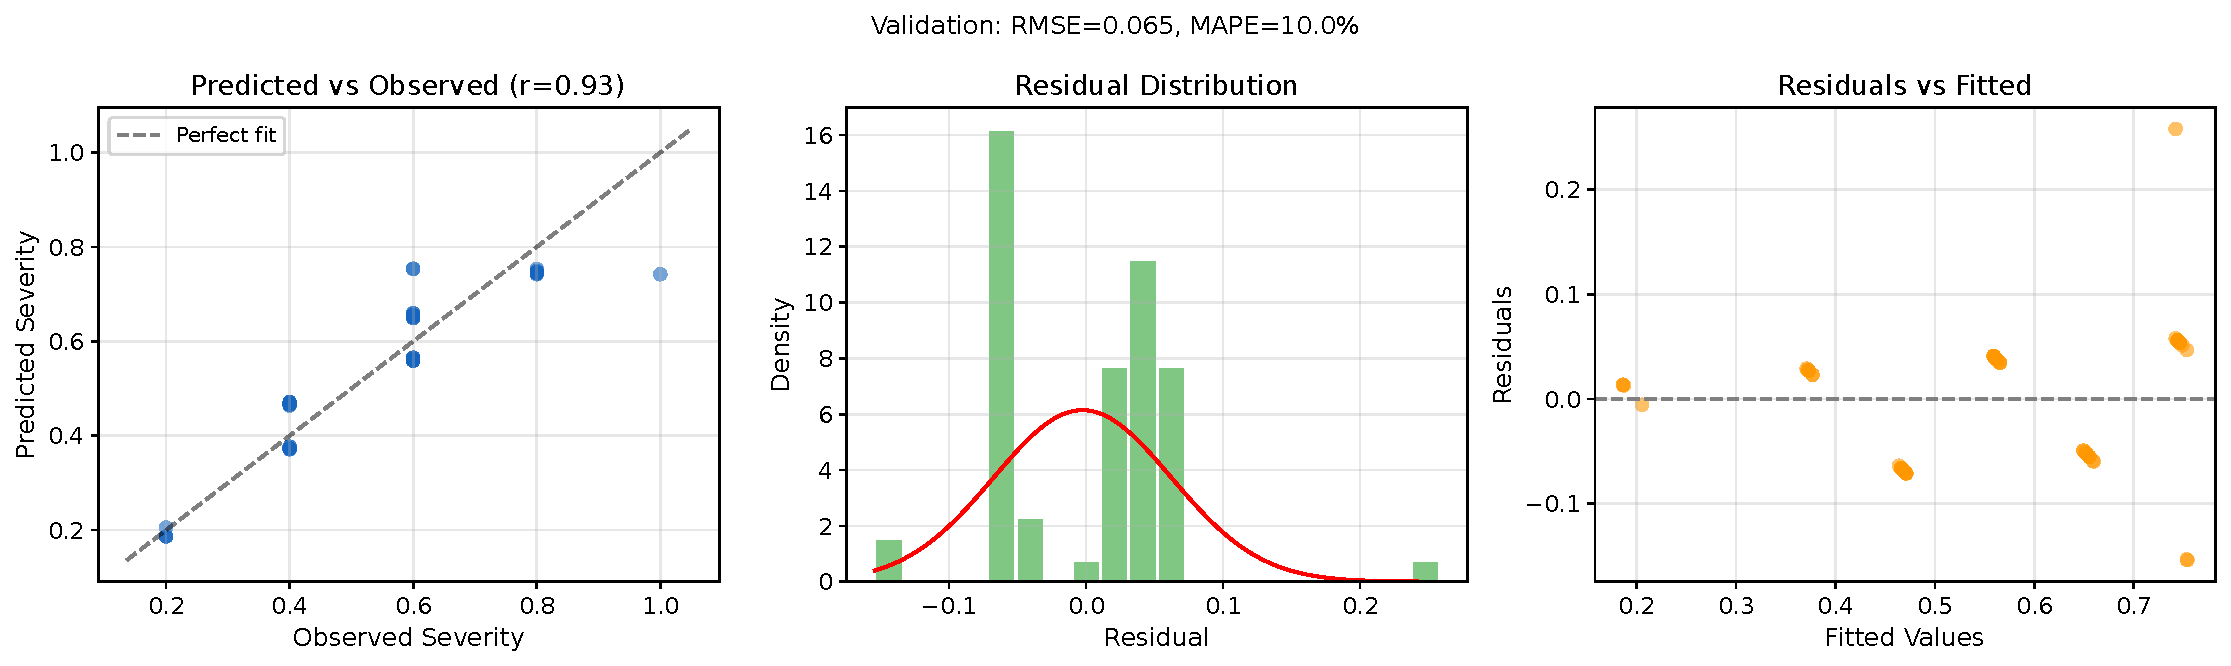
\includegraphics[width=0.82\textwidth]{residual_analysis.pdf}
\caption{Residual analysis for historical validation on the disclosed
corpus.}
\end{figure}

\end{document}
